% ---------------------------------------------------------------------------
% Timing schematic: which regime is best under the declared costs, per
% mechanism class.  Schematic only; no experimental data are shown.  The
% figure records the predeclared mechanism classes and the regime ordering each
% witness must exhibit through the real adapter before any live screen.
% ---------------------------------------------------------------------------
\begin{figure}[t]
\centering
\resizebox{\linewidth}{!}{%
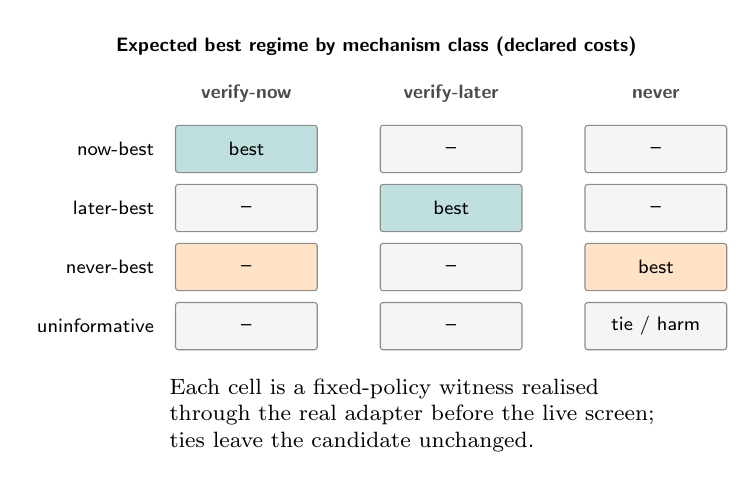
\begin{tikzpicture}[
  font=\sffamily\scriptsize,
  cell/.style={draw=black!45, rounded corners=1pt, minimum width=18mm,
               minimum height=6mm, inner sep=1pt, align=center},
  arrow/.style={-{Latex[length=1.6mm]}, line width=.5pt, black!65},
]
\node[align=center,text width=7.6cm,font=\sffamily\scriptsize\bfseries] at (1.65,2.05)
  {Expected best regime by mechanism class (declared costs)};
% header
\node[font=\sffamily\scriptsize\bfseries,text=black!70] at (0.0,1.45) {verify-now};
\node[font=\sffamily\scriptsize\bfseries,text=black!70] at (2.6,1.45) {verify-later};
\node[font=\sffamily\scriptsize\bfseries,text=black!70] at (5.2,1.45) {never};
% rows
\foreach \y/\lab in {0.75/now-best, 0.0/later-best, -0.75/never-best, -1.5/uninformative}{
  \node[anchor=east,align=right] at (-1.05,\y) {\lab};
}
\node[cell,fill=teal!25] at (0.0,0.75) {best};
\node[cell,fill=black!4] at (2.6,0.75) {--};
\node[cell,fill=black!4] at (5.2,0.75) {--};
\node[cell,fill=black!4] at (0.0,0.0) {--};
\node[cell,fill=teal!25] at (2.6,0.0) {best};
\node[cell,fill=black!4] at (5.2,0.0) {--};
\node[cell,fill=orange!22] at (0.0,-0.75) {--};
\node[cell,fill=black!4] at (2.6,-0.75) {--};
\node[cell,fill=orange!22] at (5.2,-0.75) {best};
\node[cell,fill=black!4] at (0.0,-1.5) {--};
\node[cell,fill=black!4] at (2.6,-1.5) {--};
\node[cell,fill=black!4] at (5.2,-1.5) {tie / harm};
\node[font=\footnotesize, anchor=north west, text width=6.4cm, align=left]
  at (-1.1,-2.05)
  {Each cell is a fixed-policy witness realised through the real adapter before
   the live screen; ties leave the candidate unchanged.};
\end{tikzpicture}%
}
\caption{\textbf{Timing, not ranking.}  The design asks which regime is best
under the declared costs.  Four mechanism classes are predeclared, and each is
realised by an executable fixed-policy witness through the real adapter: a world
where verifying now is best, one where reserving for checkpoint 2 is best, one
where never verifying is best, and an uninformative-or-harmful check.
\emph{Schematic: no experimental data are shown; all cells are the predeclared
target orderings, not measured outcomes.}}
\label{fig:timing}
\end{figure}
